Consider the first example.

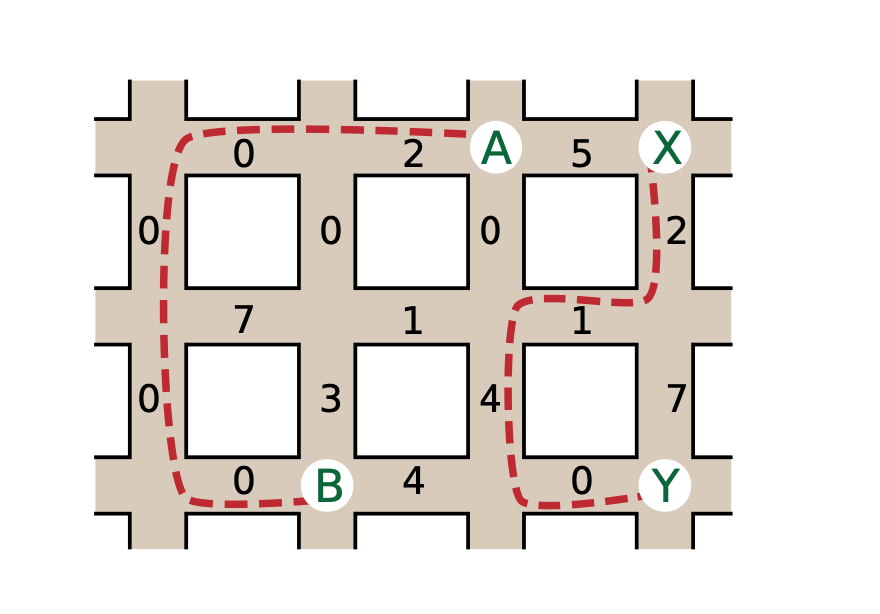
\includegraphics{wombats2.png}

The picture above shows an initial map with $R = 3$ horizontal roads and $C = 4$ vertical roads, with the number of wombats marked on each segment. Consider the following series of events:
\begin{itemize}
\item A person arrives at intersection $A = (0, 2)$ and wishes to escape to intersection $(2, 1)$. The smallest number of wombats she can pass is $2$, as indicated by a dashed line.
\item Another person arrives at intersection $X = (0, 3)$ and wishes to escape to intersection $Y = (2, 3)$. The smallest number of wombats he can pass is $7$, again indicated by a dashed line.
\item Two change events occur: the number of wombats on the top segment of vertical road $0$ changes to $5$, and the number of wombats on the middle segment of horizontal road $1$ changes to $6$. See the circled numbers in the picture below.

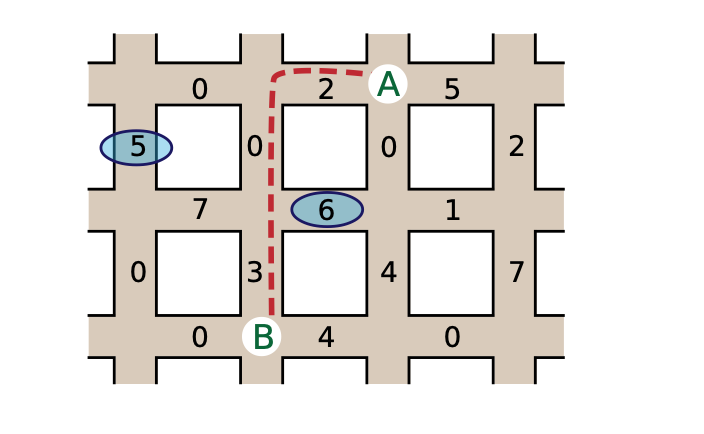
\includegraphics{wombats3.png}

\item A third person arrives at intersection $A = (0, 2)$ and wishes to escape to intersection $B = (2, 1)$. Now the smallest number of wombats she can pass is $5$, as indicated by the new dashed line.
\end{itemize}

In the file you are submitting you must \t{\#include"wombats.h"}.